\section{Face Detection}\label{sec:face-detection}
As I mentioned in the description of a facial recognition pipeline the goal of face detection is to find the location
of the face within the image.
This is challenging in unconstrained environments due to various poses, illuminations and occlusions.

To not digress too much from the main topic I will describe only the system which was put in use in the experimental
part of this thesis.
The detection algorithm is called MTCNN~\ref{subsec:mtcnn}.

Before going through the process of face detection it is necessary to describe a method called Non-maximum Suppression.

\subsection{Non-maximum Suppression}\label{subsec:nms}
Non-maximum Suppression (NMS) is a filtering algorithm of overlapping bounding
boxes\footnote{\label{foot:bbox}A rectangle describing face position.}.
NMS consists of five simple steps:
\begin{enumerate}
    \item \label{itm:nmss1}Create a list of proposal bounding boxes ordered by the confidence score.
    \item Select the bounding box with highest confidence score and add it to the filtered list of boxes.
    \item Compute IoU~\ref{fig:iou} between the selected bounding box and all the remaining ones.
    \item Remove all the boxes whose IoU is higher than some predetermined threshold.
    \item Go to~\ref{itm:nmss1} and repeat the process until there are no remaining bounding boxes within the original list.
\end{enumerate}

Having NMS defined we can proceed with actual face detection.

\subsection{MTCNN}\label{subsec:mtcnn}
MTCNN~\cite{MTCNN} stands for Multi-task Cascaded Convolutional Networks.
This model consists of three stages.

\subsubsection{Stage 1}
The first stage is called \textbf{Proposal Network} (P-Net) and its role is to find the candidate windows and their
bounding box regression vectors.
P-Net is fully convolutional neural network.

Before passing the image to P-Net we resize the image to many different sizes.
By doing so we make the model scale invariant.

Now we feed the images to the net.

The net produces many bounding boxes with a varying confidence.
We parse the output and delete the boxes with low confidence score.

Now we standardize the coordinates by converting the boxes from the coordinate systems of the resized images to
that of the unscaled one.

At this point we run NMS~\ref{subsec:nms} once for every scaled image.
Then we put all the survivors into one list and run NMS once more.

Before passing the boxes to stage 2 we make the boxes square by elongating the shorter sides.

\subsubsection{Stage 2}
The name of the second stage is \textbf{Refined Network} (R-Net).
The purpose of this stage is to filter out a large number of false positives and to calibrate the boxes.

Initially we take the boxes from the previous stage and copy the pixel values to separate arrays.
In case the box is out of bounds we fill the "empty space" with zeros.

Now we resize all the arrays to have the size of $24 \times 24$ pixels.
Currently the pixel values are in the range of $<0; 255>$ which is not optimal for the model training.
To work around the issue we normalize the values to $<-1; 1>$.

At this point we feed the images to R-Net and collect the outputs.

The outputs are similar to that of P-Net.
They also include the coordinates and the confidence levels.
The difference is that the new coordinates are more accurate.

In the last few steps of the stage 2 we remove the boxes with a lower confidence and perform NMS to remove the
redundant ones.

Now we standardize the coordinates and reshape the bounding boxes to a square.

\subsubsection{Stage 3}
In the last stage we take the boxes from stage 2 and copy the pixel values to separate arrays.
If there are any boxes which cross the image bounds we deal with then in the same way as in the previous stage.
That is we fill the empty space with zeros.

Now we resize the images to be of $48 \times 48$ pixels and feed them into a neural network called
\textbf{The Output Network} (O-Net).

O-Net is split into three layers at the top and as a result of this architectural choice produces three outputs:
the coordinates of the bounding box, the coordinates of the facial landmarks and the confidence level of each box.

In the final processing step of the whole MTCNN algorithm we get rid of the boxes with a low confidence score,
we standardize the coordinates of both the landmarks and the boxes and  we filter the boxes with NMS.

\begin{figure}[H]
    \centering
    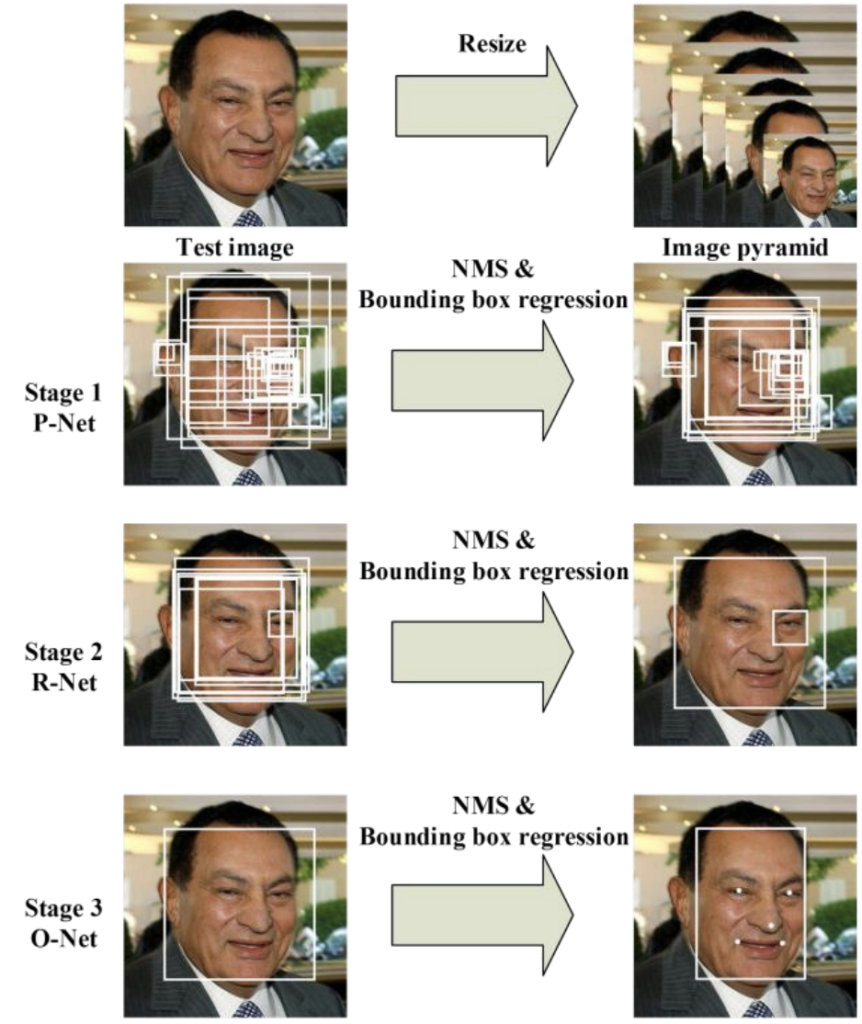
\includegraphics[width=0.7\columnwidth]{images/face-recognition/mtcnn.png}
    \caption{MTCNN face detection pipeline~\cite{MTCNN}.}
    \label{fig:mtcnn}
\end{figure}

Figure~\ref{fig:mtcnn} is a visualization of this three stage process.